\documentclass[a4paper]{article}
\usepackage{amsmath, amssymb, amsthm}
\usepackage{xcolor}
\usepackage{syntax}
\usepackage{stmaryrd}
\usepackage{float}
\usepackage{enumitem}
\usepackage{tcolorbox}
\usepackage[left=1in, right=1in, top=1in, bottom=1in]{geometry}


\AtEndPreamble{ \usepackage{hyperref} }

\usepackage[backend=biber]{biblatex}
\addbibresource{ref.bib}

\usepackage{tikz}
\usetikzlibrary{automata, arrows.meta, positioning, graphs}


\usepackage{graphicx}
\graphicspath{{figures/}, {impl/simulation-results/}}
\DeclareGraphicsExtensions{.png,PNG,.jpg,.JPG,.jpeg,.JPEG,.pdf,.PDF}

\title{Final Report: Verifying Probabilistic Program Equivalence via PGF Transformer Semantics}
\date{Finished on \today}
\author{Cheng Peng (2020533068)}

\DeclareMathOperator*{\PGF}{PGF}
\DeclareMathOperator*{\SOP}{SOP}
\DeclareMathOperator*{\VARS}{Var}
\DeclareMathOperator*{\PARMS}{Parm}
\DeclareMathOperator*{\iid}{iid}
\DeclareMathOperator*{\fix}{fix}
\renewcommand{\S}[1]{ \llbracket #1 \rrbracket }
\newcommand{\E}{ \mathbb{E} }

\newcommand{\Geom}{\mathrm{geometric}}
\newcommand{\Anno}[1]{\color{gray}{#1}}

\newtheorem{theorem}{Theorem}[section]
\newtheorem{lemma}[theorem]{Lemma}
\newtheorem{definition}[theorem]{Definition}
\newtheorem{example}[theorem]{Example}
\newtheorem{remark}[theorem]{Remark}

\begin{document}

\maketitle
% Verifying Output Distribution Equivalence for Rectangular Discrete Probabilistic Programs via the PGF transformer semantics

\begin{abstract}
	Randomness is ubiquitous in the real world, and introducing randomness is inevitable in various domains, such as machine learning and cryptography, giving rise to probabilistic programming.
	While probabilistic programming is widely applied in security-critical applications, e.g., online banking and cyber-physical systems, there is a lack of effort in ensuring their correctness.\par
	Recently, researchers proposed generating function transformer semantics to address the insufficiency of sensitivity and expressiveness of existing techniques.
	This novel denotational semantics allows tracking the entire distribution of program states, enabling precise reasoning about the behavior of probabilistic programs.\par
	In this course project, we investigate the PGF transformer semantics of the ReDiP programming language, and develop a proof-of-concept tool for equivalence checking.
\end{abstract}

\section{Introduction}

\subsection{Motivation}

% The rise of probabilistic programming
Randomness is pervasive, arising naturally and inevitably in many contexts.
For example, applications interacting with the physical world must handle noisy inputs, molecular dynamics involve stochastic motions, and random tie-breaking is crucial for efficient approximate algorithms.
In recent years, there has been a surge in probabilistic programming, which unifies statistical modelling with general-purpose programming, making it much easier to program with randomness.
\par
% The need to verify stochastic programs
Probabilistic programming is increasingly employed in safety- and security-critical applications, such as healthcare, financial services, and autonomous control systems,
where faults and vulnerabilities may lead to severe damage and significant costs. Therefore, formally verifying probabilistic programs is essential to ensure their reliability and build trust in these systems.
\par
% Insufficiency of previous works
While the need for verifying probabilistic programs is ever-growing, verification techniques are still in an early stage.
Most existing approaches focus on computing moments of variables\cite{wang2021central}, deriving probability of assertion violations\cite{assert}, or establishing lower/upper bounds\cite{probana}.
Though they are capable of detecting bugs and side-channel leaks in programs, they generally cannot determine the entire output distribution of programs,
making them insensitive to tiny deviations from the desired distribution and unable to verify complex properties such as relations between variables.
% short summary, lead to the research problem
The limitations of previous works motivate people to seek a proper theoretical foundation for precise and versatile automated reasoning of probabilistic programs.

\subsection{Overview}

This project aims to develop a verifier to determine whether two probabilistic programs generate exactly the same output distribution for every possible input.
Given that the equivalence checking problem for pGCL is undecidable, we restrict the probabilistic programming language to make equivalence decidable.
The two main restrictions we introduce are (1) arithmetic expressions must be linear, and (2) comparisons must be rectangular.
The resulting fragment is called rectangular discrete probabilistic programming language (ReDiP), a constrained yet expressive language.
It turns out that equivalence checking is decidable for ReDiP.\par
To precisely reason about probabilistic programs, a formal semantics have to be devised.
Inspired by work Kozen\cite{kozen1979semantics}, Chen et al.\cite{cav-pgf} developed a denotational semantics based on probability generating functions (PGFs) to capture the evolution of the distribution of program states as the program executes.
We investigate the PGF transformer semantics, demonstrating the recursive calculation of the PGF transform of a ReDiP program.
We also prove linearity and rational closed-form preservation of the PGF transformer semantics. Leveraging the linearity of PGF transformers of ReDiP programs, we re-implement the PRODIGY equivalence checker in Python leveraging \texttt{sympy}\cite{sympy}, a well-known computer algebra system.
Finally, we use a set of tests from PRODIGY\cite{cav-extended} to benchmark the performance and scalability of our tool.\par

The main work done in this project are:

\begin{itemize}
	\item We define the ReDiP programming language, a restricted fragment of pGCL amenable to automated reasoning.
	\item We define the PGF transformer semantics and demonstrate the forward reasoning of probabilistic programs leveraging the PGF transform semantics.
	\item We establish properties of PGF transformers of ReDiP programs and implement an equivalence verifier leveraging those properties.
	\item We benchmark our tool to show its effectiveness and discover a potential scalability issue.
\end{itemize}

\begin{figure}[htbp]
	\centering
	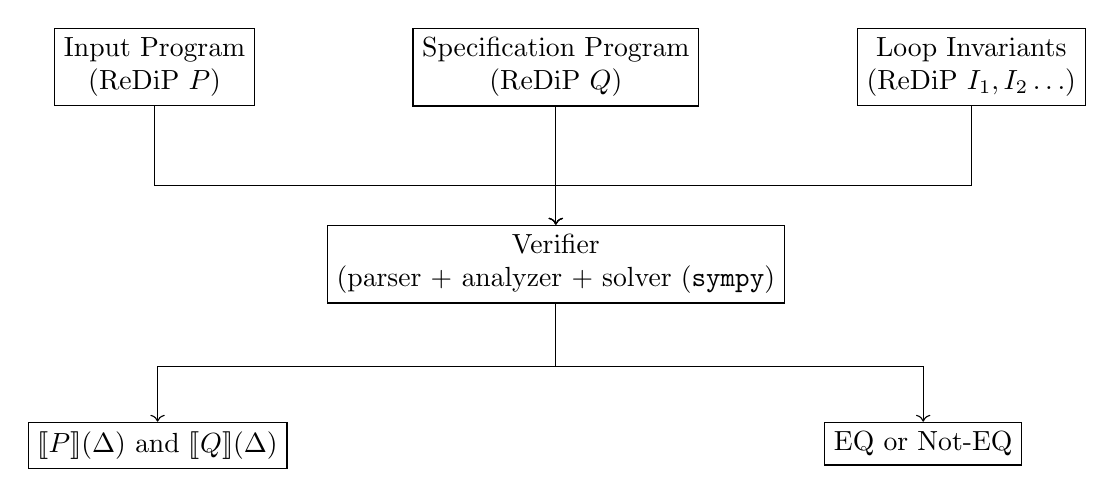
\begin{tikzpicture}[node distance=2cm, auto,
			every node/.style={rectangle, draw, text centered, minimum width=2cm, align=center}]

		% Nodes
		\node (inputProgram) {Input Program\\ (ReDiP \(P\))};
		\node (specProgram) [right=2cm of inputProgram] {Specification Program\\ (ReDiP \(Q\))};
		\node (loopInvariants) [right=2cm of specProgram] {Loop Invariants\\ (ReDiP \(I_1,I_2\ldots\))};

		\node (verifier) [below=1.5cm of specProgram] {Verifier\\ (parser + analyzer + solver (\texttt{sympy})};

		\node (output1) [below left=1.5cm and 0.5cm of verifier] {\(\S{P}(\Delta)\) and \(\S{Q}(\Delta)\)};
		\node (output2) [below right=1.5cm and 0.5cm of verifier] {EQ or Not-EQ};

		% Arrows
		\draw[->] (inputProgram.south) -- ++(0,-1) -| (verifier.north);
		\draw[->] (specProgram.south) -- (verifier.north);
		\draw[->] (loopInvariants.south) -- ++(0,-1) -| (verifier.north);

		\draw[->] (verifier.south) -- ++(0,-0.8) -| (output1.north);
		\draw[->] (verifier.south) -- ++(0,-0.8) -| (output2.north);

	\end{tikzpicture}
	\caption{Architecture of the verifier}
\end{figure}

\section{Probabilistic Programming Languages}

In this section, we introduce the syntax and semantics of the pGCL probabilistic programming language.
We later impose several reasonable constraints on pGCL to obtain a restricted yet expression language, ReDiP.

\subsection{The pGCL programming language}

The probabilistic guarded command language\cite{pgcl} is a simple imperative programming language augmented with probabilistic choice and random sampling. The syntax~\ref{def:pgcl-syn} describes what constitute a valid pGCL program, and the semantics~\ref{def:pgcl-sem} defines the step-by-step execution of a pGCL program.
\begin{definition}[pGCL syntax constructions]\label{def:pgcl-syn}
	A pGCL programn is a terminal command,
	an assignment command,
	or a compositional command, where:
	\begin{description}
		\item[terminal command] A terminal command is a \(\operatorname{skip}\) command.
		\item[assignment command] Arithmetic expression \(x:=E\). Random sampling \(x :\approx \mu\).
		\item[compositional commands] Suppose that \(C_1,C_2\) are valid pGCL programs, \(p\) is an arithmetic expression, and \(\varphi\) is a conditional (boolean) expression, then
		      \begin{itemize}
			      \item \(\{C_1\}[p]\{C_2\}\) is a probabilistic choice command
			      \item \(C_1;C_2\) is a sequencing command
			      \item \(\operatorname{if}(\varphi)\{C_1\}\operatorname{else}\{C_2\}\) is a braching command
			      \item \(\operatorname{while}(\varphi)\{C_1\}\) is a looping command
		      \end{itemize}
	\end{description}
\end{definition}

\begin{definition}[pGCL operational semantics]\label{def:pgcl-sem}
	The semantics of a pGCL program is defined as:
	\begin{itemize}
		\item A configuration space
		      \[
			      \mathcal K = \{\langle C, \sigma, n, \theta, q\rangle \mid
			      C\in p\operatorname{GCL} \cup \{\downarrow\},
			      \sigma: \Sigma\to\mathbb{Z},
			      n\in\mathbb{N},
			      \theta\in {\{L,R\}}^\ast,
			      q\in [0,1]
			      \}
		      \]
		      \begin{itemize}
			      \item \(C\) is the pGCL command to be executed or a \(\downarrow\) representing halt without error.
			      \item \(\sigma\) is the variable valuation function.
			      \item \(n\) is the number of steps up to now.
			      \item \(\theta\) records all probabilistic choices made in the past.
			      \item \(q\) is the probability of reaching such a configuration.
		      \end{itemize}
		\item A transition relation \(\vdash \subseteq \mathcal{K}\times \mathcal{K}\), defined by a set of rules:
		      \begin{itemize}
			      \item skip:
			            \(\langle \operatorname{skip},\sigma,n,\theta,q \rangle
			            \vdash
			            \langle \downarrow,\sigma,n+1,\theta,q \rangle\)
			      \item arithmetic: if \(\sigma(E)=a\) then
			            \(\langle x:=E,\sigma,n,\theta,q \rangle
			            \vdash
			            \langle \downarrow,\sigma[x\mapsto a],n+1,\theta,q \rangle\)
			      \item sampling: if \(\mu(a)=r>0\) then
			            \(\langle x:\approx\mu,\sigma,n,\theta,q \rangle
			            \vdash
			            \langle \downarrow,\sigma[x\mapsto a],n+1,\theta,qr \rangle\)
			      \item probabilistic choice:
			            If \(\sigma(p)=r>0\) then
			            \(\langle \{C_1\}[p]\{C_2\},\sigma,n,\theta,q \rangle
			            \vdash
			            \langle C_1,\sigma,n+1,\theta\cdot L, qr \rangle\)\\
			            If \(1-\sigma(p)=r'>0\) then
			            \(\langle \{C_1\}[p]\{C_2\},\sigma,n,\theta,q \rangle
			            \vdash
			            \langle C_2,\sigma,n+1,\theta\cdot R, qr' \rangle\)
			      \item sequencing:
			            If \(\langle C_1,\sigma,n,\theta,q \rangle
			            \vdash
			            \langle C_1',\sigma',n',\theta',q' \rangle \)
			            then
			            \(\langle C_1;C_2,\sigma,n,\theta,q \rangle
			            \vdash
			            \langle C_1';C_2,\sigma',n',\theta',q'\rangle\)\\
			            Also \(\langle \downarrow;C_2,\sigma,n,\theta,q \rangle
			            \vdash
			            \langle C_2,\sigma',n',\theta',q'\rangle\)
			      \item branching:
			            If \(\sigma(\varphi)=\mathbf{T}\)
			            then \(\langle \operatorname{if}(\varphi)\{C_1\}\operatorname{else}\{C_2\}=\sigma,n,\theta,q \rangle
			            \vdash
			            \langle C_1,\sigma,n+1,\theta,q\rangle\).\\
			            If \(\sigma(\varphi)=\mathbf{F}\)
			            then \(\langle \operatorname{if}(\varphi)\{P\}\operatorname{else}\{Q\}=\sigma,n,\theta,q \rangle
			            \vdash
			            \langle C_2,\sigma,n+1,\theta,q\rangle\).
			      \item looping:
			            If \(\sigma(\varphi)=\mathbf{T}\)
			            then \(\langle \operatorname{while}(\varphi)\{C\},\sigma,n,\theta,q \rangle
			            \vdash
			            \langle C;\operatorname{while}(\varphi)\{C\},\sigma,n+1,\theta,q\rangle\).\\
			            If \(\sigma(\varphi)=\mathbf{F}\)
			            then \(\langle \operatorname{while}(\varphi)\{C\},\sigma,n,\theta,q \rangle
			            \vdash
			            \langle \downarrow,\sigma,n+1,\theta,q\rangle\).
		      \end{itemize}
		      In the above paragraph,
		      \(\sigma(E)\) and \(\sigma(\varphi)\) are the value of arithmetic expression \(E\)
		      and the value of conditional expression under valuation \(\sigma\), respectively.
		\item The (possibly infinite) computation tree of program \(C\) on initial variable valuation \(\sigma\),
		      where \(k_0 = \langle C,\sigma,0,\epsilon,1\rangle\) is the root configuration.
		      The tree contains all reachable configurations. Each configuration \(k\) except for the root is linked to the configuration \(k'\) where \(k'\vdash k\).
	\end{itemize}
\end{definition}

In the end of this section, we define the terminal configurations~\ref{def:pgcl-term} of pGCL programs and formalize the intuition of equivalent programs~\ref{def:pgcl-equiv}.

\begin{definition}[Terminal configurations]\label{def:pgcl-term}
	Terminal configuration for program \(C\) on input \(\sigma_0\) is the set of all reachable halting configurations
	\[
		T(C,\sigma_0) = \left\{
		\langle \downarrow,\sigma,n,\theta,q \rangle
		\mid
		\langle C,\sigma_0,0,\epsilon,1 \rangle
		\vdash^\ast
		\langle \downarrow,\sigma,n,\theta,q \rangle
		\right\}
	\]
	The terminal valuation is defined as all possible valuation in terminal configurations.
	\[
		TV(C,\sigma_0) =
		\{\sigma \mid
		\langle \downarrow,\sigma,n,\theta,q \rangle \in T(C,\sigma_0)
		\}
	\]
	Similarly, define the terminal distribution as the probability distribution of terminal valuations.
	\[
		TD(C,\sigma_0;\sigma) = \sum_{\langle \downarrow,\sigma, n,\theta, q \rangle \in TV(C,\sigma_0)} q
	\]
\end{definition}
\begin{definition}[pGCL output equivalence]\label{def:pgcl-equiv}
	Two pGCL programs \(C_1,C_2\) are said to be equivalent if for every input \(\sigma\) the terminal distribution is identical.
	\[
		\forall \sigma_0 . \forall \sigma . TD(C_1,\sigma_0; \sigma)\equiv TD(C_2,\sigma_0;\sigma)
	\]
\end{definition}

\subsection{The Linear and Rectangula fragment of pGCL, ReDiP}

The pGCL probabilistic programming language can encode arbitrary probability Turing machine. Rice theorem suggests that there is no general sound and complete algorithm for analysing pGCL programs.
With that said, there are fragments of pGCL on which automated analysis are tractable. ReDiP is the fragment we will be working on.
\begin{definition}[ReDiP programming language]
	A ReDiP program \(C\) is a pGCL program that
	\begin{itemize}
		\item Variables in \(C\) only takes natural number values.
		\item Arithmetic expressions \(E\) in \(x:=E\) are linear.
		      They take the form \( E = y + n \)
		      where \( y,n \in \{-1,0,1\}\cup\Sigma \).
		\item Conditional expressions \(\varphi\) in
		      \(\operatorname{if}(\varphi)\{P\}\operatorname{else}\{Q\}\)
		      and
		      \(\operatorname{while}(\varphi)\{P\}\)
		      are rectangular:
		      They take the form \(\varphi = x < n\)
		      where \(x \in \Sigma\) and \(n \in \mathbb{Z}\).
	\end{itemize}
\end{definition}
To further enrich the fragment we also introduces several syntactic sugars:
\begin{itemize}
	\item Linear combination expression command
	      \[
		      x := a_0 + a_1 x_1 + a_2 x_2 \cdots a_n x_n
		      \quad
		      \text{where }
		      a_i \in \mathbb{Z},
		      x_i \in \Sigma
	      \]
	      Linear combination expressions can be expressed
	      as sequential combination of finite linear expressions.
	      For example \(x := y + 2z - 3\) is equivalent to
	      \[
		      \begin{aligned}
			      x & := y + 0; \\
			      x & := x + z; \\
			      x & := x + z; \\
			      x & := x - 1; \\
			      x & := x - 1; \\
			      x & := x - 1  \\
		      \end{aligned}
	      \]
	\item Finite loop command \(\operatorname{loop}(n)\{C\}\).
	      The command is equivalent to \(\overbrace{C;C;\cdots;C}^{n \text{ copies}}\).
	\item Logical connectives in conditional expressions: conjunction \(\varphi \land \varphi\), disjunction \(\varphi\lor\varphi\) and negation \(\lnot\varphi\).
	\item Extended rectangular conditions: \(x \langle op \rangle n\) where \(\langle op \rangle \in \{=,\neq,<,>,\leq,\geq\}\).
	\item Odd-Even conditional expression: \(x\bmod 2=0\) and \(x\bmod 2=1\).
	\item IID sampling command \(x := \iid(D,y)\) where \(D\) is a discrete probability distribution and \(x,y\) are variables.
\end{itemize}

We note that ReDiP is rich enough to write many practical programs, e.g., random walk simulation, simple rejection sampling, and Discrete Markov chains.

\section{Review on GFs and PGFs}

We first define the following notations that will be used frequently in this section:

\begin{itemize}
	\item Vectors \(\mathbf{x} = (x_1,x_2,\ldots x_k)\) and \(\sigma: \{1,\ldots,k\}\mapsto \mathbb{N}\)
	\item Monomials \(\mathbf{x}^\sigma = x_1^{\sigma(1)} x_2^{\sigma(2)} \ldots x_k^{\sigma(k)} = \prod_i x_i^{\sigma(i)}\)
	\item Formal power series (or polynomials): \(P(\mathbf{x}) = \sum_{\sigma} f(\sigma) \mathbf{x}^\sigma\) where \(f: \mathbb{N}^k\to \mathbb{R}\)
\end{itemize}

\subsection{Generating Functions}

Generating functions\cite{gfbook} (GFs) are power tools originate from the field of enumerative combinatorics.
GFs are also known as Z-transforms in the context of signal processing.
The GF of a sequnece is a formal power series whose coefficients are the elements of the sequence. For example the generating function of \(\{a_n\}\) with meta-variable \(x\) is
\[
	G(a_n; x) = \sum_{n=0}^\infty a_n x^n
\]

Manipulations on sequence can be mapped to algebraic operations on GFs.
\begin{theorem}[GF operations for sequence manipulations]
	Suppose that the GF of \(\{a_n\}\) and \(\{b_n\}\) are \(f=G(a_n,t)\) and \(g=G(b_n,t)\) respectively, then
	\begin{align*}
		G\left(a_{n-k}; x\right)                     & = x^k f              \\
		G\left(a_{n} + b_{n}; x\right)               & = f+g                \\
		G\left(r a_{n}; x\right)                     & = r f                \\
		G\left(\sum_{k=0}^{n} a_{k}b_{n-k}; x\right) & = fg                 \\
		G\left(n a_n; x\right)                       & = x \partial_x f     \\
		G\left(a_{n-1}/n; x\right)                   & = \int f \mathrm{d}x \\
	\end{align*}
\end{theorem}

\begin{table}[htbp]
	\label{tab:gf-close}
	\[
		\begin{array}{l|l|l}
			\hline
			\text{Generating function }g(x) & \text{sequence }[x^n]g(x) & \text{note}             \\
			\hline
			(1-ax)^k                        & \binom{k}{n}a^n           & a,k\in\mathbb{R}^{\ast} \\[2ex]
			(1-x)^{-1}                      & 1                         &                         \\[2ex]
			(1-x)^{-2}                      & n+1                       &                         \\[2ex]
			x^k                             & [n=k]                     & k\in\mathbb{N}^{+}      \\[2ex]
			e^{kx}                          & k^n/n!                    & k\in\mathbb{R}^{\ast}   \\[2ex]
			-\ln(1-x)                       & 1/n                       & n\geq 1                 \\[2ex]
			\hline
		\end{array}
	\]
	\caption{Elementary generating functions and their corresponding sequences}
\end{table}
Certain formal power series have equivalent elementary closed-form representation, they can be regarded as finite representation of infinite sequences. Table~\ref{tab:gf-close} summarizes typical closed-form GFs.
Working on closed-form of generation functions of sequences is easy, since elementary functions are closed under arithmetics, composition, and differentiation.
Furthermore, indefinite integration of elementary functions can be computed via the Risch algorithm if the result is elementary.\par
The following example demonstrates the use of generating function in solving linear recurrence relations.

\begin{example}[Problem solving using GFs]
	Find the closed-form formula of \(u_n\) where
	\[
		\begin{cases}
			u_0 = v_1 = 1            \\
			v_0 = u_1 = 0            \\
			u_n = 2v_{n-1} + u_{n-2} \\
			v_n =  u_{n-1} + v_{n-2} \\
		\end{cases}
	\]
	Let \(U(z)\) and \(V(z)\) be the generating function of the two sequences, then
	\[
		\begin{cases}
			U(z) = 1 + 2z V(z) + z^2 U(z) \\
			V(z) = zU(z)+z^2U(z) = \frac{z}{1-z^2}U(z)
		\end{cases}
	\]
	Solve the equation system to get the closed-form of \(U(z)\), which is a rational function:
	\[
		U(z)={\frac {1-z^{2}}{1-4z^{2}+z^{4}}}={\frac {1}{3-{\sqrt {3}}}}\cdot {\frac {1}{1-\left(2+{\sqrt {3}}\right)z^{2}}}+{\frac {1}{3+{\sqrt {3}}}}\cdot {\frac {1}{1-\left(2-{\sqrt {3}}\right)z^{2}}}
	\]
	Thus
	\[
		U_{2n+1} = 0 \qquad U_{2n} = \left\lceil \frac{(2+\sqrt 3)^n}{3-\sqrt 3} \right\rceil
	\]
\end{example}

Generating functions of sequences can be extended to represent higher-dimensional sequences.
For example, the generating function of the 2D sequence \(a_{n,m}\) with meta-variables \(x\) and \(y\) is
\[
	G(a_{n,m}; x,y) = \sum_n \sum_m a_{n,m} x^n y^m
\]
In general, the generating function for a \(k\)-dimensional sequence \(f:\mathbb{N}^k\to\mathbb{R}\) has the following form
\[
	G(f; \mathbf{x}) = \sum_{\sigma \in \mathbb{N}^k} f(\sigma) \mathbf{x}^\sigma
\]

\subsection{Probability Generating Functions}

The PGF of a non-negative discrete random variable \(X\) is defined as
\[
	g_X(t) = \E(t^X) = \sum_{n=0}^\infty \Pr(X=n) t^n
\]
It can be regarded as the Z-transform of the probability mass function.
PGFs provides concise representation of probability distributions, greatly simplifying probabilistic reasoning. Table~\ref{tab:pgfs}

\begin{table}[htbp]
	\centering
	\begin{tabular}{l|l|l}
		\hline
		Distribution                         & Probability Mass Function                                         & PGF                                                     \\
		\hline
		\(\operatorname{Bernoulli}(p) \)     & \( \Pr(X = 1) = p, \ \Pr(X = 0) = 1 - p \)                        & \( 1 - p + pz \)                                        \\[2ex]
		\(\operatorname{Binomial}(n, p) \)   & \( \Pr(X = k) = \binom{n}{k} p^k (1 - p)^{n - k} \)               & \( (1 - p + pz)^n \)                                    \\[2ex]
		\(\operatorname{Geometric}(p) \)     & \( \Pr(X = k) = (1 - p)^{k - 1} p \)                              & \( \frac{pz}{1 - (1 - p)z} \)                           \\[2ex]
		\(\operatorname{Poisson}(\lambda) \) & \( \Pr(X = k) = \frac{\lambda^k e^{-\lambda}}{k!} \)              & \( e^{\lambda(z - 1)} \)                                \\[2ex]
		\(\operatorname{DUnif}(a, b) \)      & \( \Pr(X = k) = \frac{1}{b - a + 1} \) for \( k = a, \ldots, b \) & \( \frac{z^a(1 - z^{b - a + 1})}{(b - a + 1)(1 - z)} \) \\[2ex]
		\(\operatorname{NBin}(r, p) \)       & \( \Pr(X = k) = \binom{k + r - 1}{k} (1 - p)^r p^k \)             & \( \left( \frac{pz}{1 - (1 - p)z} \right)^r \)          \\[2ex]
		\hline
	\end{tabular}
	\caption{PGFs of Common Distributions}
	\label{tab:pgfs}
\end{table}

\begin{theorem}[PGF of the linear transform of a variable]
	Let \(X\) be a random variable whose PGF is \(g_X(t)\).
	Then the PGF of \(Y=aX+b\) is \(g_Y(t) = t^b g_X(t^a)\)
	\[
		g_Y(t)
		= \E(t^{aX+b})
		= \E({(t^a)}^X \cdot t^b)
		= t^b \E({(t^a)}^X )
		= t^b g_X(t^a)
	\]
\end{theorem}
\begin{theorem}[PGF of the sum of two independent variables]
	Let \(g_X(t)\) and \(g_Y(t)\) be the generating function of two independent random variables \(X\) and \(Y\), respectively. Then the PGF of \(Z=X+Y\) is \(g_Z(t) = g_X(t)g_Y(t)\)
	\[
		g_Z(t) = \E(t^Z) = \E(t^X t^Y) = \E(t^X) \E(t^Y) = g_X(t) g_Y(t)
	\]
\end{theorem}
\begin{theorem}[PGF of random stopping sum]
	Let \(X_1, X_2, \ldots\) be a sequence of iid variables with PGF \(g_X(\cdot)\),
	and \(N\) be a independent random variable with PGF \(g_N(\cdot)\).
	Then, \(S=\sum_{i=1}^{N} X_i\) has PGF \(g_S = g_N\circ g_X\).
	\begin{align*}
		\E_{N,\mathbf{X}}\left\{ t^{\sum_{i=1}^N X_i} \right\}
		 & = \E_N\left\{ \E_{\mathbf{X}|N}\left[ t^{\sum_{i=1}^N X_i} \mid N \right] \right\}
		= \E_N\left\{ \E_{\mathbf{X}|N}\left[ \prod_{i=1}^N t^{X_i} \mid N \right] \right\}     \\
		 & = \E_N\left\{ \prod_{i=1}^N \E_{\mathbf{X}|N}\left[  t^{X_i} \mid N \right] \right\}
		= \E_N\left\{ \prod_{i=1}^N \E_{\mathbf{X}}\left[  t^{X_i} \right] \right\}
		= \E_N\left\{ {(g_X(t))}^N \right\}                                                     \\
		 & = \sum_{n=0}^{\infty} {(G_X(t))}^n \Pr(N=n)
		= g_N(g_X(t))
	\end{align*}
\end{theorem}

Finally, PGFs can be generalized to work with random vectors.
For example, the PGF of \((X,Y)\sim p(x,y)\) is
\[
	g_{X,Y}(s,t) = \E(s^X t^Y) = \sum_{n=0}^\infty \sum_{m=0}^\infty \Pr(X=n,Y=m) s^n t^m
\]
In general, for a \(k\)-dimensional random vector \(\mathbf{X}=(X_1,X_2,\ldots X_k)\), the PGF is defined as
\[
	g_{\mathbf{X}}(\mathbf{t}) = \E(\mathbf{t}^\mathbf{X}) = \sum_{\sigma\in\mathbb{N}^k} \Pr(\mathbf{X}=\sigma) \mathbf{t}^\sigma
\]

\section{PGF transformer semantics}

The small-step operational semantics provides a micro-level view program execution, focusing on the state evolution over one particular execution path. While this approach is suitable for deriving fine-grained properties of a program, it lacks the capability to capture the overall behavior of the program.
Denotational semantics, on the other hand, offers a holistic view by representing collections program states with mathematical objects and mapping program execution to transformations of these objects.
The PGF transformer semantics represents the distribution over all reachable program states as a PGF. The semantics of a program is then modelled as a transformer that maps one PGF to another PGF.

\begin{example}[PGF of distribution over program states]
	Consider the following ReDiP program
	\[
		N := 1; M :\approx \operatorname{Poisson}(1/2)
	\]
	For any initial program state distribution, the terminal program state distribution is always
	\[
		p(n,m) = [m=3] \binom{9}{n}\frac{1}{2^n \times 2^{9-n}}
	\]
	In PGF transformer semantics, the program transforms any input state distribution PGF \(g=\E(s^N t^M)\) into \({\left( \frac12 + \frac12 s \right)}^s t^3\), denoted as
	\[
		\S{N := 1; M :\approx \operatorname{Poisson}(1/2)}
		= g\mapsto {\left( \frac12 + \frac12 s \right)}^s t^3
	\]
\end{example}

\subsection{PGF transformer of loop-free ReDiP program}

The PGF transformer semantics of ReDiP programs is defined as follows:
\begin{definition}[PGF transformer of a ReDiP program]
	For a ReDiP program \(P\), let \((X_1,X_2,\ldots,X_k)\) be all the variables used in a \(P\),
	then the PGF transformer \(\S{P}\) is a \(\PGF\to\PGF\) mapping such that:
	\begin{enumerate}
		\item For every distribution \(\mu_0\) over the possible program state \(\mathbb{N}^k\).
		      Let \(g(\mathbf{t}) = \E_{\mathbf{X}\sim\mu_0}(\mathbf{t}^\mathbf{X})\) be the PGF of \(\mathbf{X}\sim\mu_0\).
		\item If the initial program state \(\sigma_0\) is sampled from \(\mu_0\): \(\sigma_0 \sim \mu_0\).
		\item The terminal program state distribution \( \mu_1(\sigma_1) = \E_{\sigma_0\sim \mu_0}\left[ TD(C,\sigma_0;\sigma_1) \right] \)
		      should satisfy \(\S{P}(g) = h\) where \(h(\mathbf{t}) = \E_{\mathbf{Y}\sim\mu_1}(\mathbf{t}^\mathbf{Y})\) is the PGF of \(\mathbf{Y}\sim\mu_1\).
	\end{enumerate}
\end{definition}
We now explain how to compute PGF transformers of ReDiP programs.
For the sake of simplicity, we assume that the program contains only two variables \(x\) and \(y\) and the PGF of program state distribution is \(g=\E(s^X t^Y)=\sum_{x,y} p(x,y) s^x t^y\).
\begin{theorem}[PGF transformers of non-conditional pGCL commands]
	The PGF transformers for skip command, linear arithmetic commands, and random sampling commands:
	\begin{itemize}
		\item \(\S{\operatorname{skip}} = id\) since a skip command does not change the program states.
		\item \(\S{x := 0} = g\mapsto g[s/1]\) since \( g[s/1] = \E(1^X t^Y) = \E(t^Y) = \E(s^0 t^Y) \)
		\item \(\S{x := x+n} = g\mapsto s^n g\) since \( s^n g = s^n \E(s^X t^Y) = \E(s^n s^X t^Y) = \E(s^{X+n} t^Y) \)
		\item \(\S{x := x+y} = g\mapsto g[t/st]\) since \( g[t/st] = \E(s^X {(st)}^Y) = \E(s^X s^Y t^Y) = \E(s^{X+Y} t^Y) \)
		\item \(\S{x := x-1} = g\mapsto g[s/0] + s^{-1}(g-g[s/0])\) since
		      \[
			      \mathbb{E}(s^{\max(0,X-1)} t^Y) =
			      \sum_y p(0,y) s^0 t^y + \sum_{x\geq 1} \sum_y p(x,y) s^{x-1} t^y
			      = g[s/0] + s^{-1}(g-g[s/0])
		      \]
		\item \(\S{x :\approx \mu} = g\mapsto g[s/1] h(s)\) where \(h(s) = \E_{Z\sim \mu}(s^Z)\).
		      \[
			      g[s/1] h(s)
			      = \E(t^Y) \E_{Z\sim \mu}(s^Z)
			      = \E_{Z\sim \mu}(s^Z t^Y)
			      = \E_{X\sim \mu}(s^X t^Y)
		      \]
		\item \(\S{x := x+\iid(\mu,y)} = g\mapsto g[t/t h(s)]\) where \(h(s) = \E_{Z\sim \mu}(s^Z)\).
		      \begin{align*}
			      g[t/t h(s)] & = \E(s^X {(t h(s))}^Y) = \E(s^X {(h(s))}^Y t^Y)                        \\
			                  & = \E_{Z_1,Z_2\ldots\stackrel{\iid}{\sim}\mu}(s^X s^{\sum_{i=1}^Y} t^Y)
			      = \E_{Z_1,Z_2\ldots\stackrel{\iid}{\sim}\mu}(s^{X+\sum_{i=1}^Y} t^Y)
		      \end{align*}
	\end{itemize}
	The PGF transformers of several other ReDiP language constructions which does not involves conditional branching can also be computed:
	\begin{itemize}
		\item \(\S{C_1;C_2} = \S{C_2}\circ \S{C_1}\)
		\item \(\S{\{C_1\}[p]\{C_2\}} = g\mapsto p \S{C_1}(g) + (1-p)\S{C_2}(g)\)
		\item \(\S{\operatorname{loop}(n)\{C\}} = \S{C}\circ \S{C} \cdots \S{C}\) where \(\S{C}\) is repeated n times.
		\item \(\S{x := x-n} = \S{\operatorname{loop}(n)\{x := x-1\}}\)
	\end{itemize}
\end{theorem}
To work with conditional expressions, we define the filtered PGFs.
\begin{definition}[Filtered PGFs]
	For \(g = \E(s^X t^Y)\) the \(k\)-th Taylor term of \(g\) with respect to \(s\), \(tt(g,s,n)\), is define as
	\[
		tt(g,s,n) = \frac{s^k}{k!}\left(\frac{\partial^k g}{\partial s^k}[s/0]\right)
	\]
	Filtered PGF is defined as \(g_{\varphi} = \E([\varphi(x,y)]s^X t^Y)\) where \(\varphi(x,y)\in \{0,1\}\) is called the filtering condition.
	The exclusive prefix filtered PGF: \(g_{x<n}\) for \(n\in\mathbb{N}\) can be computed as
	\[
		g_{x<n} = \sum_{x<n}\sum_y p(x,y) s^x t^y = \sum_{k<n} tt(g,s,k)
	\]
	Based on \(g_{x<n}\) several other filtered PGFs can be computed:
	the inclusive prefix \(g_{x\leq n} = g_{x<n+1}\),
	the exclusive suffix \(g_{x>n} = g - g_{x\leq n}\),
	and the inclusive suffix \(g_{x\geq n} = g_{x>n-1}\).
	Furthermore \(g_{2\mid x}\) and \(g_{2\nmid x}=g-g_{2\mid x}\) can also be efficiently computed:
	\[
		g + g[s/(-s)]
		= \E(s^X t^Y) + \E({(-s)}^X t^Y)
		= \E((1 + {(-1)}^X) s^X t^Y)
		= \E(2[2\mid X] s^X t^Y)
		= 2 g_{2\mid x}
	\]
	For compositional propositions \(\varphi \land \psi\), \(\varphi\lor \psi\), and \(\lnot \varphi\), their corresponding filtered PGF can be computed recursively:
	\begin{itemize}
		\item Negation \(g_{\lnot \varphi} = g-g_{\varphi}\)
		\item Conjunction \(g_{\varphi \land \psi} = h_{\psi}\) where \(h = g_{\varphi}\)
		\item Disjunction \(g_{\varphi \lor \psi} = g_{\lnot (\lnot \varphi \land \lnot \psi)}\)
	\end{itemize}
\end{definition}
Transformers of branching and looping commands can be computed by leveraging filtered PGFs:
\begin{theorem}[PGF transformer of if commands]
	\(
	\S{\operatorname{if}(\varphi)\{C_1\}\operatorname{else}\{C_2\}} =
	g\mapsto \S{C_1}(g_{\varphi}) + \S{C_2}(g_{\lnot \varphi})
	\)
\end{theorem}

\subsection{PGF transformer of loops}

Unbounded loops are characterized as least fixed point in denotational semantics.
To define least fixed points, we need a partial order \((\sqsubseteq, \PGF)\).
\begin{definition}[Partial order of PGFs]
	Let \(f\) and \(g\) be the PGFs of two \(k\)-dimensional discrete random vectors, where
	\[
		f = \sum_{\sigma} f(\sigma) \mathbf{t}^\sigma
		\qquad
		g = \sum_{\sigma} g(\sigma) \mathbf{t}^\sigma
	\]
	We say \(f \sqsubseteq g\) if and only if \(\forall \sigma . f(\sigma) \leq g(\sigma)\).
\end{definition}
This partial order is shown to be a \(\omega\)-complete partial order\cite{cav-extended}.
Now that the PGF space is equipped with a partial order, we characterize loops with fixed points.
\begin{theorem}[PGF transformer of while commands]
	\(\S{\operatorname{while}(\varphi)\{C\}} = \mu\ Q . \operatorname{if}(\varphi)\{C;Q\}\)\\
	That is, the least fixed point of the function \(Q \mapsto \operatorname{if}(\varphi)\{C;Q\}\).
\end{theorem}
Intuitively, a while loop is equivalent to a infinitely nested branching tree, which ultimately converges if the loop always terminate.
\begin{tcolorbox} \begin{verbatim}
while(cond){
    body;
}\end{verbatim}
\end{tcolorbox}

\begin{tcolorbox} \begin{verbatim}
if(cond){ body;
if(cond){ body;
if(cond){ body;
  ....
}
}
}
\end{verbatim}
\end{tcolorbox}

\begin{tcolorbox} \begin{verbatim}
least_fix_point((Q) => {
    if (cond) {body; Q}
})
\end{verbatim}
\end{tcolorbox}

The least fixed point characterization of while loops completes the last piece of the PGF transformer semantics of ReDiP.
However a general algorithm that computes least fixed does not exists.
In stead of finding the fixed point, we ask the fixed point to be given as part of the input.
The only work left to be done is to check whether the given program \(Q\) is indeed the fixed point of \(Q\mapsto \operatorname{if}(\varphi)\{C;Q\}\).
\begin{definition}[Probabilistic termination]
	A pGCL program \(P\) is said to be universally almost-surely terminating (UAST),
	if for every initial configuration \(\langle P,\sigma,0,\epsilon,1 \rangle\) it evolves to a halting configuration, i.e., a configuration of the form \(\langle \downarrow, \sigma', n,\theta,q\rangle\), with probability 1.
\end{definition}

\begin{theorem}[Fixed point induction]\label{thm:lfp-ind}
	Let \(\operatorname{while}(\varphi)\{C\}\) be a ReDiP loop, then
	\[
		\S{\operatorname{if}(\varphi)\{C;Q\}\operatorname{else}\{\operatorname{skip}\}} \sqsubseteq \S{Q}
		\implies
		\S{\operatorname{while}(\varphi)\{C\}} \sqsubseteq \S{Q}
	\]
	Furthermore, if the loop is UAST, then
	\[
		\S{\operatorname{if}(\varphi)\{C;Q\}\operatorname{else}\{\operatorname{skip}\}} = \S{Q}
		\iff
		\S{\operatorname{while}(\varphi)\{C\}} = \S{Q}
	\]
	That is: the fixed point for a loop is the loop invariant.
\end{theorem}
To check whether \(Q\) is the least fixed point of \(\operatorname{while}(\varphi)\{C\}\):
\begin{enumerate}
	\item Check if the loop is UAST with an external tool.
	\item Check if \(\S{\operatorname{if}(\varphi)\{C;Q\}\operatorname{else}\{\operatorname{skip}\}} = \S{Q}\).
	      The two programs are both loop-free ReDiP.
	      We will discuss how to determine equivalence of loop-free ReDiP programs later.
\end{enumerate}
Theorem~\ref{thm:lfp-ind} is a special case of Park's induction. Detailed proof can be found in the PRODIGY paper\cite{cav-extended}.

\subsection{Properties of ReDiP PGF transformers}

In this section, we prove two important properties of ReDiP PGF transformers, which enables efficient equivalence checking algorithms.
The general approach for proving properties of ReDiP PGF transformers is structure induction over the program.

\begin{theorem}[linearity]
	For every ReDiP program \(P\), and two PGFs \(f,g\).
	\[
		\forall \lambda\in[0,1] . \S{P}(\lambda f + (1-\lambda) g) = \lambda \S{P}(f) + (1-\lambda)\S{P}(g)
	\]
\end{theorem}
\begin{proof}
	Without lose of generality, we consider only two-dimensional PGFs.
	For two PGFs \(f,g\) and two non-negative real numbers \(a,b\) where \(a+b=1\).
	\begin{enumerate}
		\item Base case: PGF transformers of atomic commands are linear.
		      \begin{enumerate}
			      \item \(x := 0\) transformer \(g\mapsto g[s/1]\)
			            \[
				            (af + bg)[s/1] = a(f[s/1]) + b(g[s/1])
			            \]
			      \item \(x := x+n\) transformer \(g\mapsto s^n g\)
			            \[
				            (af + bg) \mapsto (af + bg)s^n = a(s^n f) + b(s^n g)
			            \]
			      \item \(x := x+y\) transformer \(g\mapsto g[t/st]\)
			            \[
				            (af + bg) \mapsto (af + bg)[t/st] = a(f[t/st]) + b(g[t/st])
			            \]
			      \item \(x :\approx \mu\) transformer \(g\mapsto g[s/1]h(s)\) where \(h(\cdot)\) is the PGF of \(\mu\).\\
			            The transformer is the composition of \(g\mapsto g[s/1]\) and \(g\mapsto g h(s)\) which are both linear,
			            so the resulting mapping is linear.
			      \item \(x := \iid(\mu,y) \) transformer \(g\mapsto g[s/1][t/th(s)]\) where \(h(\cdot)\) is the PGF of \(\mu\).\\
			            The transformer \(g\mapsto g[t/t h(s)]\) is linear
			            \[
				            (af + bg) \mapsto (af + bg)[t/t h(s)] = a(f[t/t h(s)]) + b(g[t/t h(s)])
			            \]
			            The transformer \(\S{x := \iid(\mu,y)}\) is the composition of \(g\mapsto g[s/1]\) and \(g\mapsto g[t/t h(s)]\) which are both linear, so the resulting mapping is linear.
		      \end{enumerate}
		\item Induction case: Suppose that \(P,Q\) are ReDiP programs whose PGF transformers are linear.
		      \begin{enumerate}
			      \item \(P;Q\) transformer \(g\mapsto \S{Q}(\S{P}(g))\).
			            \[
				            (af+bg) \mapsto \S{Q}(a\S{P}(f) + b\S{Q}(g)) = a\S{Q}(\S{P}(g)) + b \S{Q}(\S{P}(g))
			            \]
			      \item \(\{P\}[p]\{Q\}\) transformer \(g\mapsto p\S{P}(g) + (1-p)\S{Q}(g)\).
			            \begin{align*}
				            (af+bg) & \mapsto  p\S{P}(af+bg) + (1-p)\S{Q}(af+bg)                                             \\
				                    & = ap\S{P}(f) + bp\S{P}(g) + a(1-p)\S{Q}(f) + b(1-p)\S{Q}(g)                            \\
				                    & = a\left(p\S{P}(f) + (1-p)\S{Q}(f)\right) + b\left( p\S{P}(g) + b(1-p)\S{Q}(g) \right) \\
			            \end{align*}
			      \item \(\operatorname{if}(\varphi)\{P\}\operatorname{else}\{Q\}\) transformer \(g\mapsto \S{P}(g_{\varphi}) + \S{Q}(g_{\lnot\varphi})\)\\
			            We can verify that the PGF filtering operators are linear.
			            \begin{align*}
				            (af+bg) & \mapsto \S{P}(a f_{\varphi} + b g_{\varphi}) + \S{Q}(a f_{\varphi} + b g_{\varphi})                                           \\
				                    & = a\S{P}(f_{\varphi}) + b\S{P}(g_{\varphi})  + a\S{Q}(f_{\lnot\varphi}) + b\S{Q}(g_{\lnot\varphi})                            \\
				                    & = a\left( \S{P}(f_{\varphi}) + \S{Q}(f_{\lnot\varphi}) \right) + b\left( \S{P}(g_{\varphi}) + \S{Q}(g_{\lnot\varphi}) \right)
			            \end{align*}
			      \item \(\operatorname{while}(\varphi)\{P\}\) transformer \(\mu\ Q . \operatorname{if}(\varphi)\{P;Q\}\)\\
			            Intuitively, a while loop is a infinitely nested branching tree.
			            Considering PGF transformers of if-branchings are linear, the PGF transformer of nested branching tree should also be linear.
			            Rigorous proof of this need to properties of \(\omega\)-complete partial order. The proof is omitted and can be found in\cite{cav-extended}.
		      \end{enumerate}
	\end{enumerate}
\end{proof}

\begin{definition}[rational closed-forms]
	\(f\in\PGF\) is said to be in rational closed-form if
	\[
		f = \frac{g}{h} = \dfrac{
			\sum_{\sigma \leq a^k} g(\sigma) \mathbf{t}^\sigma
		}{
			\sum_{\sigma \leq b^k} h(\sigma) \mathbf{t}^\sigma
		}
		\quad
		a,b \in \mathbb{N}
	\]
	That is, the \(f\) is the quotient of two finite polynomials.
\end{definition}

\begin{theorem}[rational closed-form preservation]
	For a loop-free ReDiP program \(P\), and a rational-closed form PGF \(g/h\),
	there exists two finite polynomials \(g',h'\) such that \(\S{P}(g/h) = g'/h'\).
\end{theorem}
\begin{proof}
	Without lose of generality, we consider only two-dimensional PGFs.
	For two PGFs \(f,g\) and two non-negative real numbers \(a,b\) where \(a+b=1\).
	\begin{enumerate}
		\item Base case: PGF transformers of atomic commands preserve rational-closed form.\\
		      This is because rational-closed forms are closed under compositor and linear combination.
		      Note that substituting a variable with a constant/monomial/rational function is essentially composing the input PGF with a rational function.
		      The detailed case-analysis is omitted.
		\item Induction case: PGF transformers of compositional commands preserve rational-closed form.\\
		      This is because rational-closed form preserving mappings is closed under composition and linear combination.
		      The detailed case-analysis is omitted.
	\end{enumerate}
\end{proof}

Rational closed-forms are amenable to computer algebra systems, e.g., \texttt{sympy} and \texttt{GiNaC}.
The rational closed-form preservation property allow us to efficiently compute \(\S{P}(g/h)\) for a loop-free program \(P\).
Furthermore, rational functions have simple normal forms (sort the monomials in lexicographical order), so deciding rational functions equivalence is very easy.\par
Finally, we note that the closed-form preservation property is of more theoretical interest than practical significance.
Our tool has support for sampling from a PGF specified by a elementary function, so our tool is actually working on elementary closed-form rather than rational closed-form.
Though computations involving arbitrary elementary functions do not have simple and clear complexity bound, computer algebra systems are often able to compute the results in reasonable time (for example, 10 seconds).

\section{Deciding Equivalence of loop-free ReDiP programs}

As we have seen in previous section, fixed point induction allow transforming a loopy ReDiP programs into a semantically equivalent loop-free programs when a correct loop invariant is supplied,
so the problem of deciding equivalence of ReDiP programs can be reduced to deciding equivalence of loop-free ReDiP programs.
Now consider the problem of checking whether two ReDiP programs \(P,Q\) are equivalent. Suppose that the program state of both programs is a random vector \((X_1,X_2,\ldots X_k)\).
\begin{enumerate}
	\item By definition, we have to check if:
	      \[
		      \forall \sigma_0 . \forall \sigma . TD(P,\sigma_0; \sigma)\equiv TD(Q,\sigma_0;\sigma)
	      \]
	\item By encode the initial and terminal program states with PGFs,
	      the distribution equivalence problem is reduced to a PGF transformer equivalence problem:
	      \[
		      \forall g\in \PGF(X_1,\ldots X_k) . \S{P}(g) = \S{Q}(g)
	      \]
	\item By linearity of PGF transformers of ReDiP programs, we only need to check if \(\S{P}(\cdot)\) and \(\S{Q}(\cdot)\) are consistent on a basis of \(\PGF(X_1,\ldots X_k)\).
	      One of such basis is the set of all point-mass distribution.
	      Every distributions \(p(\mathbf{X})\) over \(\mathbb{N}^k\) can be expressed as a linear combination of point-mass distributions:
	      \[
		      p(\mathbf{x}) = \sum_{\mathbf{y}\in\mathbb{N}^k} p(\mathbf{y}) \delta_{\mathbf{y}}(\mathbf{x})
		      \quad
		      \delta_{\mathbf{y}}(\mathbf{x}) = \begin{cases}
			      1 & \mathbf{x} = \mathbf{y}    \\
			      0 & \mathbf{x} \neq \mathbf{y} \\
		      \end{cases}
	      \]
	      Thus, the problem is reduced to check if:
	      \[
		      \forall \mathbf{x} \in \mathbb{N}^k \quad \S{P}(\mathbf{t}^{\mathbf{x}}) = \S{Q}(\mathbf{t}^{\mathbf{x}})
	      \]
	      where \(\mathbf{t}^{\mathbf{x}} = \sum_{\mathbf{y}\in\mathbb{N}^k} \delta_{\mathbf{x}}(\mathbf{y}) \mathbf{t}^{\mathbf{y}}\) is the PGF of the point-mass distribution \(\delta_{\mathbf{x}}(\cdot)\).
	\item Note that there are infinitely many point-mass PGFs (monomials), so the equivalence check cannot be performed by a computer algebra systems.
	      To address this, we embed all \(k\)-dimensional point-mass PGFs into a \(2k\)-dim PGF by introducing \(k\) extra meta-variables.
	      \[
		      \Delta(\mathbf{t};\mathbf{u})
		      = \sum_{y_1,y_2,\ldots y_n} (u_1 t_1)^{y_1}(u_2 t_2)^{y_2}\cdots (u_n t_n)^{y_n}
		      = \prod_{i=1}^n \left( \sum_{j=0}^\infty (t_i u_i)^j \right)
		      = \prod_{i=1}^n (1-t_i u_i)^{-1}
	      \]
	      \(\Delta\) is a so-called second-order PGF (SOP) since it can be regarded as a formal power series with meta-variable \(\mathbf{u}\),
	      where the coefficient of \(\mathbf{u}^{\mathbf{x}}\) is the PGF of \(\delta_{\mathbf{x}}(\cdot)\).
	      \begin{align*}
		      \forall \mathbf{x} \in \mathbb{N}^k \quad \S{P}(\mathbf{t}^{\mathbf{x}}) = \S{Q}(\mathbf{t}^{\mathbf{x}})
		       & \iff
		      \sum_{\mathbf{x}\in\mathbb{N}^k} \S{P}(\mathbf{t}^{\mathbf{x}}) \mathbf{u}^\mathbf{x}
		      = \sum_{\mathbf{x}\in\mathbb{N}^k} \S{Q}(\mathbf{t}^{\mathbf{x}}) \mathbf{u}^\mathbf{x}              \\
		       & \iff
		      \S{P}\left( \sum_{\mathbf{x}\in\mathbb{N}^k} \mathbf{t}^{\mathbf{x}} \mathbf{u}^\mathbf{x} \right)
		      = \S{Q}\left( \sum_{\mathbf{x}\in\mathbb{N}^k} \mathbf{t}^{\mathbf{x}} \mathbf{u}^\mathbf{x} \right) \\
		       & \iff \S{P}(\Delta(\mathbf{t};\mathbf{u}))
		      = \S{Q}(\Delta(\mathbf{t};\mathbf{u}))
	      \end{align*}
	      Therefore, the equivalence checking problem is ultimately reduced to check if \(\S{P}\) and \(\S{Q}\) agree on one PGF, \(\Delta\), which has a rational-closed form.
\end{enumerate}

In summary, to check if two loop-free ReDiP programs \(P,Q\) are equivalent, we first compute \(\Delta\) and then compare \(\S{P}(\Delta)\) and \(\S{Q}(\Delta)\).

\section{Evaluation}

\emph{Statement of data availability}: Our implementation, benchmark suite, and benchmark results are made publicly available.
The artifacts are hosted on a Github repository \href{https://github.com/hehelego/prodigy-replica}{https://github.com/hehelego/prodigy-replica}.

\subsection{Experiment setup}

We implemented the aforementioned equivalence checking algorithm in about 500 lines of Python code. All algebraic computations are carried out by \texttt{sympy}\cite{sympy}, a famous long-establish computer algebra system written in Python.\par
To test the correctness and measure the efficiency of our tool, we measured the running time of our tool on 15 pairs of programs available in the PRODIGY repository. The PRODIGY repository also contains benchmark for symbolic Bayesian inference, which is unrelated to equivalence checking. To get insight into the scalability of our tool, we also made a benchmark of 10 programs with finite loop of \(1,2,3,\ldots 10\) iterations.
\begin{verbatim}
nat x; x := geometric(1/2);
loop(n){ // number of iterations
 if(x > 15){ {x := x+1}[1/2]{x := x-1} }{}
}
\end{verbatim}
The experiments were conducted on a laptop equipped with a 8-core x86-64 CPU (model AMD RYZEN 4800U) and 16GB of DDR4 memory.

\subsection{Results}

The test results are summarized in table~\ref{tab:test1} and table~\ref{tab:test2}.
The results show that our tool can correctly and efficiently verify equivalence of a various practical ReDiP programs.
However, the scalability is unsatisfying figure~\ref{fig:test2} suggests that the verification time may grow exponentially as the program size grows.


\begin{table}[htbp]
	\centering
	\begin{tabular}{llll}
		\hline
		Test case                        & Expected result & Result         & Time  \\
		\hline
		dep_bern.pgcl                    & equivalent      & equivalent     & 6.81s \\
		dueling_cowboys_parameter.pgcl   & equivalent      & equivalent     & 4.61s \\
		geometric.pgcl                   & equivalent      & equivalent     & 2.62s \\
		geometric_observe.pgcl           & equivalent      & equivalent     & 2.72s \\
		geometric_observe_parameter.pgcl & equivalent      & equivalent     & 4.90s \\
		geometric_parameter.pgcl         & equivalent      & equivalent     & 4.45s \\
		geometric_shifted.pgcl           & equivalent      & equivalent     & 6.18s \\
		ky_die.pgcl                      & equivalent      & equivalent     & 18.5s \\
		ky_die_2.pgcl                    & equivalent      & equivalent     & 3.96s \\
		n_geometric.pgcl                 & equivalent      & equivalent     & 2.37s \\
		negative_binomial_parameter.pgcl & equivalent      & equivalent     & 4.07s \\
		random_walk.pgcl                 & equivalent      & equivalent     & 4.46s \\
		running_paper_example.pgcl       & equivalent      & equivalent     & 2.36s \\
		trivial_iid.pgcl                 & equivalent      & equivalent     & 1.85s \\
		ky_die_parameter.pgcl            & not equivalent  & not equivalent & 26.0s \\
		\hline
	\end{tabular}
	\caption{Correctness test}\label{tab:test1}
\end{table}

\begin{table}[htbp]
	\centering
	\begin{tabular}{l|llllllllll}
		\hline
		iterations & 1     & 2      & 3      & 4      & 5      & 6      & 7      & 8      & 9       & 10      \\
		\hline
		time       & 2.75s & 10.90s & 19.36s & 30.84s & 43.52s & 58.54s & 72.68s & 90.30s & 105.35s & 122.72s \\
		\hline
	\end{tabular}
	\caption{Scalability test}\label{tab:test2}
\end{table}

\begin{figure}
	\begin{center}
		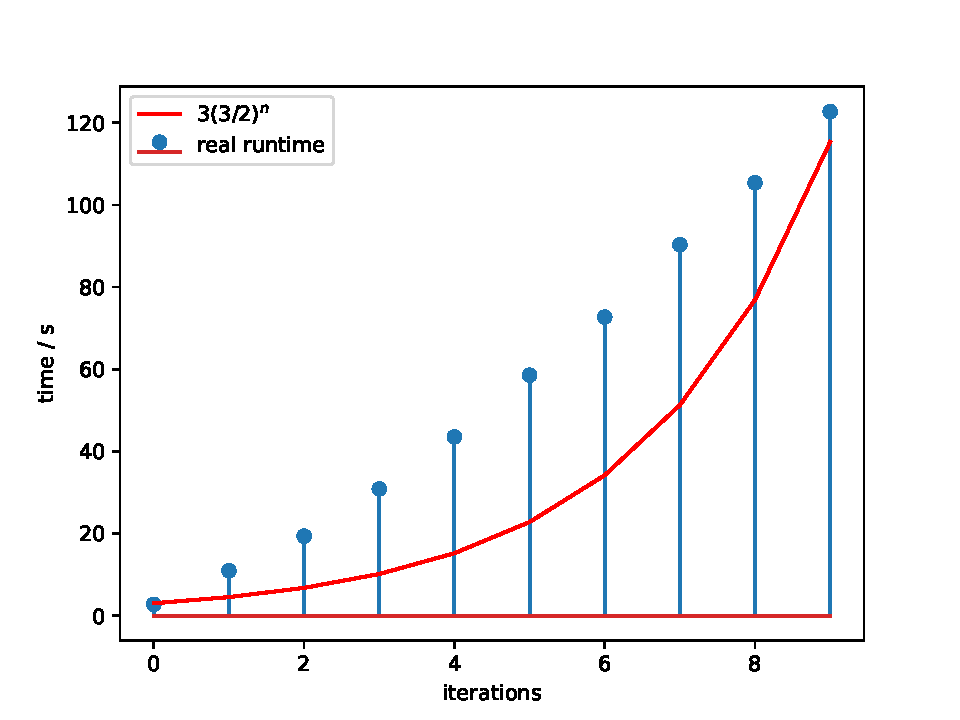
\includegraphics[width=0.95\textwidth]{scale}
	\end{center}
	\caption{Visualization of scalability test result}\label{fig:test2}
\end{figure}

\subsection{Case Study: loop invariant checking}

In this section, we give a step-by-step demonstration of the \texttt{n\_geometric.pgcl} example.\par
First, consider the following ReDiP program. We can manually derive the PGF transformer of it.
Let \( g  = \sum_{i=0}^\infty s^i h_i \), where \(h_i = \frac{1}{i!}\frac{\partial^i g}{\partial s^i}[s/0]\), be the input PGF

\begin{align*}
	 & \Anno{Input \gets g = \E(s^n t^c)}                                                          \\
	 & \operatorname{while} (n>0) \{  \Anno{g_1 = g - g[s/0] }                                     \\
	 & \quad \{ n := n - 1 \} \Anno{g_2 = g_1 s^{-1}}                                              \\
	 & \quad [1/2]                                                                                 \\
	 & \quad \{ c := c + 1 \} \Anno{g_3 = g_1 t}                                                   \\
	 & \quad \Anno{g_4 = \frac12 (g_2 + g_3)}                                                      \\
	 & \} \Anno{Output \gets \mu \left[ g \mapsto g[s/0] + \frac12(s^{-1} + t)(g-g[s/0]) \right] } \\
\end{align*}
In this case, the least fixed point do have a neat closed form:
\begin{enumerate}
	\item Suppose \(f\) is the LFP, then \( f = f[s/0] + \frac12(s^{-1} + t)(f-f[s/0]) \), which implies \(f = f[s/0]\). Therefore every term in the LFP is \(s\)-free.
	\item The term \(s^0 h_0\) never changes. As for \(s^i h_i\), where \(i>0\):
	      \begin{enumerate}
		      \item It gets multiplied by \(t/2\) or \(s^{-1}/2\), until it becomes a \(s\)-free term.
		      \item Suppose that it becomes a \(s\)-free term after \(i+j\) iterations:
		            The last factor must be \(s^{-1}/2\), and \(j\) factors among the other \(i+j-1\) factors are \(t/2\).
		            Therefore
		            \[
			            s^i h_i \rightsquigarrow h_i 2^{-i} \binom{i+j-1}{j} 2^{-j}t^j = \binom{-i}{j}2^{-j} t^j
		            \]
		      \item Take the summation over \(j=0,1,2\ldots\)
		            \[
			            \frac{h_i}{2^i} \sum_{j=0}^\infty \binom{-i}{j} 2^{-j}t^j
			            = \frac{h_i}{2^i} {(1-t/2)}^{-i}
		            \]
	      \end{enumerate}
	\item Thus, the least fixed-point is
	      \[
		      g\mapsto h_0 + \sum_{i=1}^\infty \frac{h_i}{2^i} {(1-t/2)}^{-i}
		      = \sum_{i=0}^\infty \frac{h_i}{2^i} {(1-t/2)}^{-i}
		      = g[s/{(1-t/2)}^{-1}]
	      \]
\end{enumerate}
Considering that \(g\mapsto g[s/{(1-t/2)}^{-1}] = \S{c := c + \iid(\Geom(1/2),n)}\),
the program should be semantically equivalent to the following loop-free ReDiP program denoted by \(I\)

\begin{align*}
	 & \Anno{Input \gets g = \E(s^n t^c)}                                                 \\
	 & \operatorname{if} (n>0) \{ \Anno{g_1 = g-g[s/0]}                                   \\
	 & \quad c := c + \iid(\Geom(1/2),n) ; \Anno{g_2 = g_1[s/s {(1-t/2)}^{-1}]}           \\
	 & \quad n := 0 \Anno{g_3 = g_2[s/1] = g_1[s/{(1-t/2)}^{-1}]}                         \\
	 & \} \Anno{Output \gets g[s/0] + (g-g[s/0])[s/{(1-t/2)}^{-1}] = g[s/{(1-t/2)}^{-1}]} \\
\end{align*}

To check if the loopy version and the loop-free version are equivalent,
we first apply fixed point induction to get the following program denoted by \(J\)
\begin{align*}
	 & \operatorname{if} (n > 0) \{                               \\
	 & \quad \Anno{\text{// loop body}}                           \\
	 & \quad \{n := n-1\}[1/2]\{c := c+1\}                        \\
	 & \quad \Anno{\text{// supplied loop invariant/fixed-point}} \\
	 & \quad \operatorname{if} (n > 0) \{                         \\
	 & \qquad c := c + \iid(\Geom(1/2),n);                        \\
	 & \qquad n := 0                                              \\
	 & \quad \}                                                   \\
	 & \}                                                         \\
\end{align*}

We then check if \(\S{I}(\Delta)=\S{J}(\Delta)\) where \(\Delta = {(1-s u)}^{-1} {(1-t v)}^{-1}\) for meta-variables \(s-u\) and \(t-v\).
Our tool automatically gives the following results\footnote{The real \texttt{n\_geometric.pgcl} uses an additional variable \texttt{tmp}}

\begin{itemize}
	\item Variables \(\{c\mapsto u_0x_0, n\mapsto u_1x_1, tmp\mapsto u_2x_2\}\).
	\item For the transformed program:
	      \texttt{(-u1*(u2*x2 - 1) + (u2 - 1)*(u1 + x0 - 2)) \\ / ((u2 - 1)*(u0*x0 - 1)*(u2*x2 - 1)*(u1 + x0 - 2))}
	\item For the spec program:
	      \texttt{-u1/(u0*u1*u2*x0 - u0*u1*x0 + u0*u2*x0**2 - 2*u0*u2*x0 \\ - u0*x0**2 + 2*u0*x0 - u1*u2 + u1 - u2*x0 + 2*u2 + x0 - 2) \\ + 1/((u0*x0 - 1)*(u2*x2 - 1))}
	\item Outputs are equivalent.
	\item Finished in \texttt{2.320946780964732} seconds.
\end{itemize}

\section{Conclusion and Discussion}

So far, we have demonstrated the PGF transformer semantics of a simple probabilistic programming language,
explained how the novel denotational semantics can be used to perform equivalence checking,
built a tool for ReDiP equivalence verification,
and tested it on small-scale inputs.\par

\subsection{Limitations and Future Work}

\subsubsection{Conditional reasoning}
Many probabilistic programming languages provides conditional feature for Bayesian inference.
For example, the following program should compute \(\E(Z - X + Y\mid X^2+Y^2 < Z^2)\) where \(X,Y,Z\stackrel{\iid}{\sim}\mathcal{N}(0,1)\).

\begin{align*}
	 & x,y,z :\approx (normal(0,1),normal(0,1),normal(0,1)); \\
	 & \operatorname{observe}(x^2 + y^2 < z^2);              \\
	 & s := z - (x + y);                                     \\
	 & x := 0; y := 0; z := 0;                               \\
\end{align*}

How to augment the PGF transformer semantics to enable conditional reasoning is a future research direction of theoretical interest and practical value.

\subsubsection{Incorporating Continuous Random Variables using MGF/CF}
Many statistical models and stochastic processes involve real-valued random variable, and practical probabilistic programming languages often have support for continuous random variable.
However, ReDiP only support integer-valued discrete random variable.
It remains to be explore how to add support for common distributions like \(\mathcal{N}(\mu,\sigma^2)\) and \(\beta(\alpha,\beta)\).\par

One possible attempt is to use characteristic functions (CF) or moment generating functions (MGF) instead of probability generating functions (PGF).
CF/MGF enjoys nice properties like linearity and convolution theorem. Furthermore, CF of constant assignments and linear arithmetics can be easily expressed:
\begin{align*}
	\S{x:= c}   & = g\mapsto c^s g[s/0] & e^{cs} \E(e^{0X + tY}) & = \E(e^{sc + tY})     \\
	\S{x:= x+y} & = g\mapsto g[t/(s+t)] & \E(e^{sX + (t+s)Y})    & = \E(e^{s(X+Y) + tY}) \\
	\S{x:= ax}  & = g\mapsto g[s/as]    & \E(e^{(sa)X + tY})     & = \E(e^{s(aX) + tY})  \\
\end{align*}
However, it remain unclear how can we efficiently compute the prefix-filtered CF/MGF:
\[
	\varphi_{x<c}(t) = \E(t^{i[X<c]X}) = \int_{-\infty}^c f(x) e^{itx} \mathrm{d}x
\]

\subsubsection{Verifying Reactive Programs}

Our approach relies on fixed point induction to handle unbounded loops. Fixed point induction requires the program to be UAST.
Therefore, we can only correctly compute the PGF transformer of UAST programs.\par
In reactive programs (or streaming programs) process infinite data stream perpetually. These programs never terminate.
For example, consider the following two programs. Our tool cannot determine whether they are equivalent or not.

\noindent \begin{minipage}[t]{0.45\textwidth}
	\begin{tcolorbox}
		\begin{verbatim}
setCallback((input) => {
  [a1, a2] := iid(std_normal, 2)
  x[n] := input;
  output(a1 * (x[n-1] - mu)
        + a2 * (x[n-2] - mu)^2);
  mu := (mu*n + x[n]) / (n+1);
  n = n + 1;
})\end{verbatim}
	\end{tcolorbox}
\end{minipage}
\hspace{2ex}
\begin{minipage}[t]{0.45\textwidth}
	\begin{tcolorbox}
		\begin{verbatim}
setCallback((input) => {
  [a1, a2] := iid(std_normal, 2)
  output(a1 * x[n-1]
        + a2 * x[n-2]^2);
  x[n] := input - mu;
  n := n + 1
  mu := (mu*n + x[n]) / n
})\end{verbatim}
	\end{tcolorbox}
\end{minipage}

In the future, one might explore how PGF transformers semantics can be used to verify equivalence of reactive programs.

\appendix
\setlength{\parskip}{0pt}
\nocite{*}
\printbibliography

\end{document}
